\part{Noções Básicas}

\section{Introdução do Capítulo}

Neste capítulo vamos falar sobre o porquê, para começo de conversa, devemos saber como nos proteger no mundo digital. Também vamos explicar o básico para que você consiga entender diversos conceitos com mais facilidade nas próximas páginas do livro.

\chapter{Princípios}

\section{A Informação}

A Sociedade global está passando por uma alta evolução tecnológica. Carros estão começando a se dirigir sozinhos, drones estão praticamente em toda gravação na indústria cinematográfica, O GPS do celular baixa o mapa de qualquer cidade que você está e te mostra o caminho até o lugar que você quiser e até mesmo aparelhos mais inusitados como sua geladeira podem estar conectados na internet é um fato do mundo de hoje. Todas essas coisas geram, buscam ou interpretam \textbf{informação}, uma coisa que virou uma grande riqueza no mundo globalizado.

Basta você ver qualquer documento de Termos de Serviços online que você lê (Ou deveria ler) quando se inscreve em algo na internet. Em muitos deles é dito que as suas informações produzidas no serviço são utilizadas para aprimorar ele mesmo, ou então para "oferecer propagandas mais relevantes", ou até são vendidas para outras empresas que usam estes dados para diversas outras coisas. As suas informações de uso de um app, detalhes que você coloca em um post de uma rede social produzem riquezas para outras pessoas. 

A importância da informação na verdade já existe há centenas de anos. A espionagem praticamente existe há séculos para poder obter uma vantagem militar, uma fofoca no emprego pode ser usada para conseguir um aumento no salário, atrapalhar um colega chato, ou descobrir a fórmula secreta de outra lanchonete para fazer um sanduíche melhor. Tudo isso consiste em conseguir (seja de forma moral ou imoral) uma informação que vai ser preciosa para você.

Há, portanto, um conflito de interesses. A privacidade não é um direito da pessoa? Como ela vai conseguir se proteger? No Brasil a \textbf{LGPD} (Lei Geral de Proteção de Dados \cite{lgpd}), que será comentada mais adiante, protege a privacidade do brasileiro. Na outra direção, diversas empresas e sociedades buscam proteger suas próprias informações, estabelecendo regras para seus empregados e investindo em segurança.

\begin{figure}[htb]
    \centering
    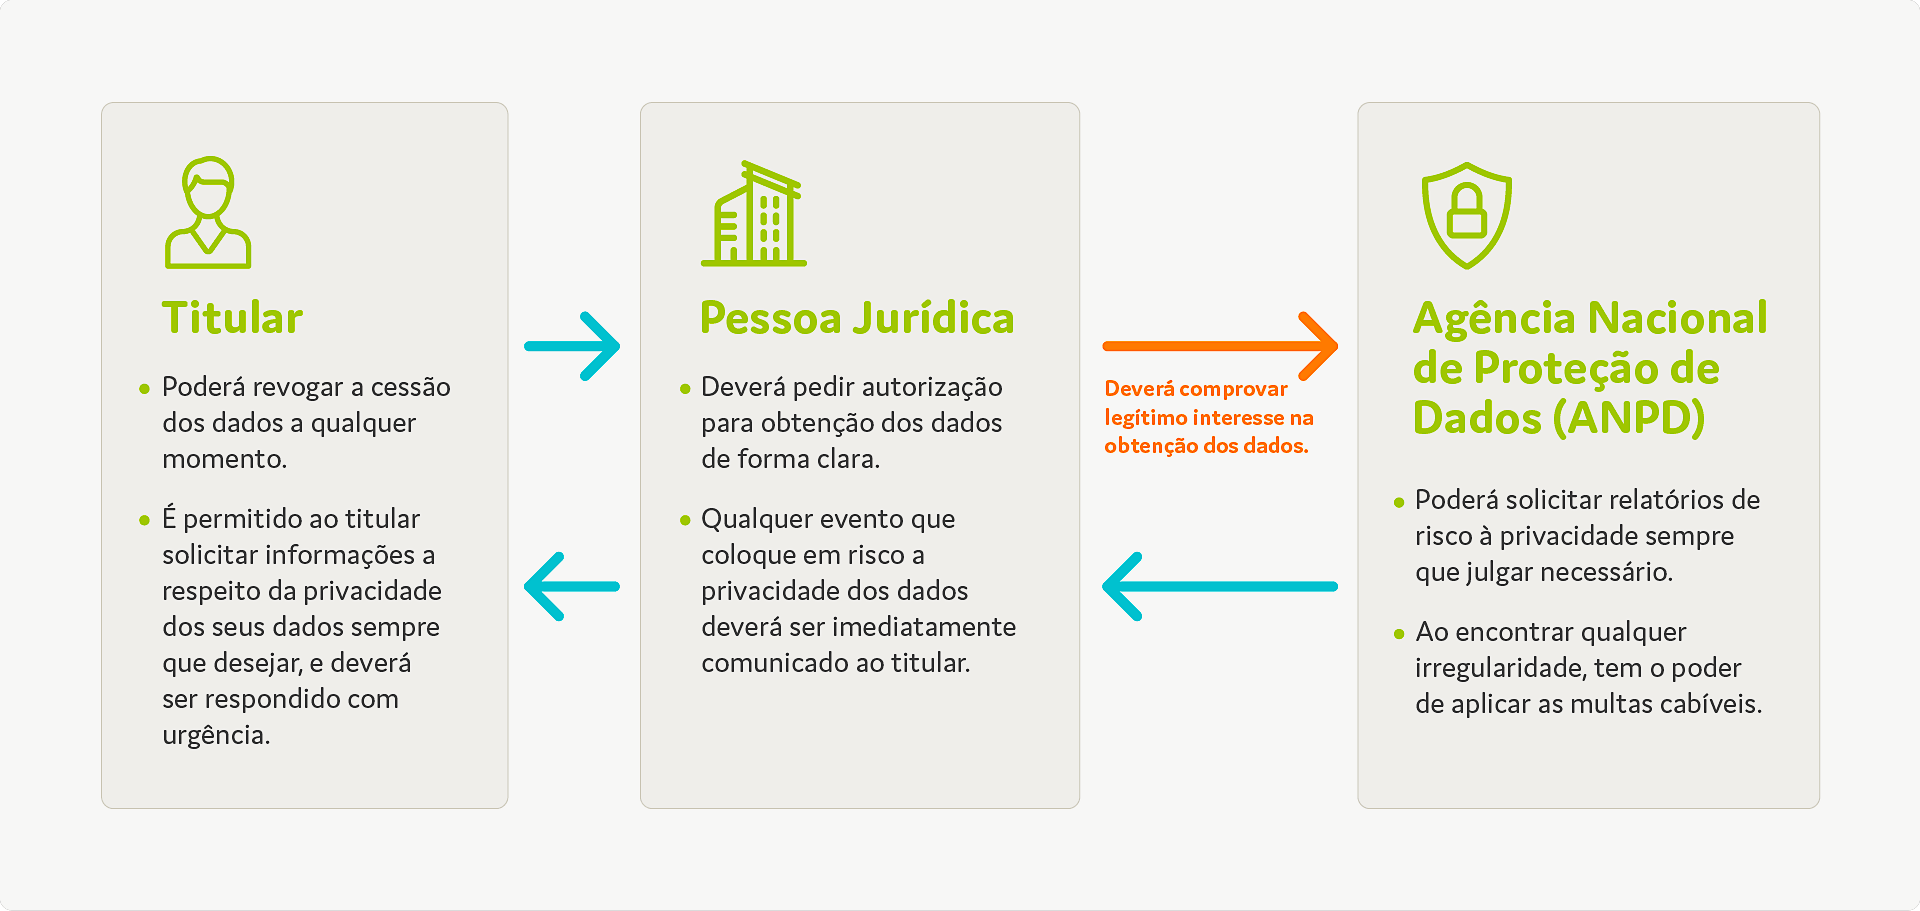
\includegraphics[width=\textwidth]{img/lgpd.png}
    \caption{Alguns dos direitos oferecidos pela LGPD. Fonte: \cite{senior}}
    \label{fig:lgpddireitos}
\end{figure}

\subsection{A Segurança}

Todo mundo tem algo que quer proteger. Com a informação é a mesma coisa. O termo "Segurança da Informação" é bem abrangente e pode ser definido de diversas formas. O vazamento de dados pode ser uma tragédia, trazendo prejuízos tanto a uma pessoa física, quanto a uma empresa.

Na revolução industrial a segurança da informação era pouco pensada como é hoje. Para se ter acesso aos dados de uma fábrica você precisava ir fisicamente nela e roubar documentos reais que provavelmente ficavam relativamente bem guardados. Hoje em dia as empresas tem bancos de dados digitais que podem ser acessados em qualquer ponto no globo desde que você saiba a forma correta de acessá-lo. Dado o tamanho de muitas dessas bases de dados é possível imaginar que levaria muito tempo para conseguir todas, mas não. Os dados digitais tem muita flexibilidade e em pouco tempo uma cópia completa de muitos gigabytes pode ser produzida e colocada em um pen-drive. Proteger esses dados é um investimento que muitas empresas fazem (ou deveriam fazer).

Para uma pessoa normal esse tipo de segurança se traduz em proteger as suas senhas como a do banco ou a de uma rede social. Além de levar em consideração o que a pessoa oferece ou coloca de informação na internet um outro aspecto deve ser observado: O que a pessoa consegue de informação na internet. Fake news e alguns métodos de ataques cibernéticos dependem da falta de conhecimento ou ignorância do funcionamento do mundo digital.


\subsection{Segurança da Informação}

Existe uma norma internacional de proteção da informação, a ISO/IEC 17799, que define os seguintes princípios

\begin{itemize}
    \item Confidencialidade: Somente pessoas autorizadas podem acessar informações, ou seja, houve uma permissão de acesso.
    \item Disponibilidade: Garante o acesso à informação na mesma hora para quem for acessá-la. Ou seja, o sistema e a rede que oferece esses dados deve funcionar perfeitamente.
    \item Integridade: As informações não podem ser adulteradas, no sentido de terceiros mal intencionados mudando dados para se favorecer.
\end{itemize}

Também temos que considerar que os dados produzidos devem ser legais e autênticos, ou seja, os dados foram produzidos obedecendo as leis e que quando comunicados ou enviados essas informações não foram alteradas no meio do caminho.

Em uma empresa esses princípios são observados pelo setor de Segurança da informação. Ele irá interagir com quase todos os outros setores da empresa exigindo que regras sejam observadas.

A mesma idéia pode ser usada para uma pessoa. Definindo regras e seguindo observações, ela terá poucos problemas relacionados a vazamento de dados.


\section{Incidentes de segurança}

Para explicar a violação de segurança precisamos entender o que é um Ativo. O Ativo é qualquer coisa que tenha valor para alguém e caso ele seja roubado ou violado teremos impactos negativos. É um termo bem abrangente, sua carteira é um ativo, pessoas podem ser também, seu celular, uma garrafa térmica de café etc..

A violação de segurança vai afetar negativamente o nosso ativo e essa violação pode se dar de diversas formas. Uma má operação, um ataque cibernético, desastres, falhas, são todas ameaças aos nossos ativos. Reconhecer ameaças e tentar evitá-las é uma grande tarefa.

Sabendo disso podemos começar a entender o que são ameaças à informação.

\subsection{Ameaças}

\begin{figure}[htb]
    \centering
    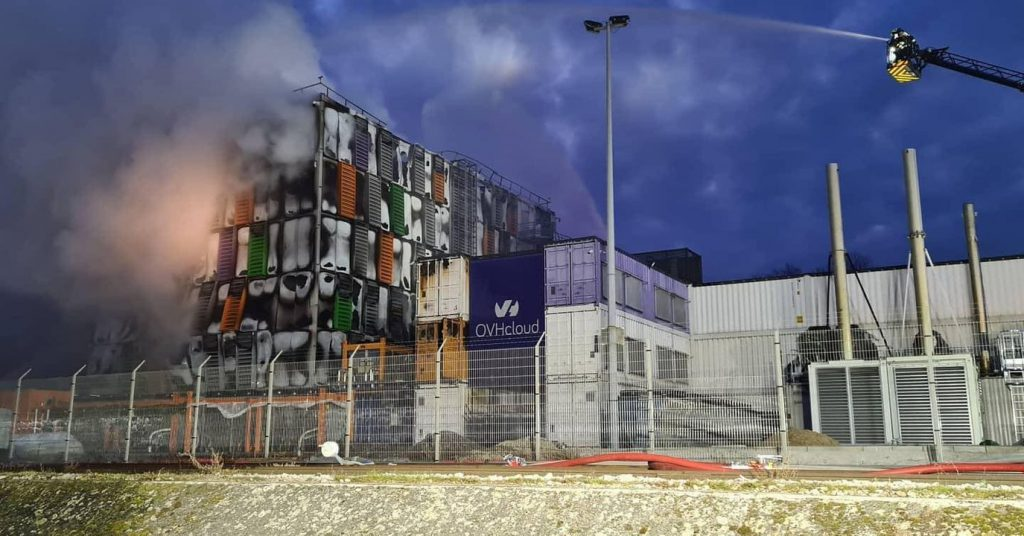
\includegraphics[width=\textwidth]{img/incendio.jpeg}
    \caption{Imaginar seu computador pegando fogo pode ser algo engraçado, mas é algo que pode acontecer. Este data center na França não teve tanta sorte e 3,6 milhões de sites ficaram fora de ar. Fonte:\cite{incendio}}
    \label{fig:incendio}
\end{figure}

Uma vulnerabilidade a um ativo da informação pode se dar das formas citadas antes, má operação, ataque, desastre, etc... E podemos separá-las em duas categorias:

\begin{itemize}
    \item Físico: Ameaças realmente físicas. Terremotos, incêndios, descargas elétricas, entre outras, nos computadores ou servidores de uma instituição;
    \item Lógico: Ameaças no mundo virtual: Vazamento de senhas, malwares, ransonwares, sites fingindo ser outros, etc...
\end{itemize}

\begin{figure}[htb]
    \centering
    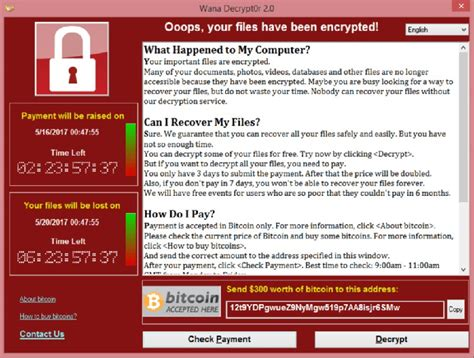
\includegraphics[width=\textwidth]{img/wannacry.jpg}
    \caption{Screenshot de um vírus de computador que ficou famoso. Esse é um tipo de vírus chamado ransonware, que encripta os arquivos pessoais do computador e exige um pagamento anônimo em criptomoeda para desencriptar.}
    \label{fig:wannacry}
\end{figure}

A forma com que se dão também podem se dividir em outras categorias:

\begin{itemize}
    \item Natural: Terremotos, tempestades, raios, enchentes
    \item Involuntárias: Ameaças inconsistentes. Acidentes de trabalho, alguém tropeçando em um fio importante, clicando um botão que não devia. Em resumo: o ator do incidente não teve a intenção de causar problemas.
    \item Intencional: Alguém quis causar problemas. Esses podem ser espiões, criminosos, invasores ou até mesmo alguém que não tenha nenhuma razão em especial.
\end{itemize}

\subsection{Vulnerabilidade}

Qualquer falha que o sistema possui e que pode dar problema. Digamos que você escreva suas senhas em um caderno. Se você deixa o caderno na cozinha existe a possibilidade de cair alguma bebida em cima dele e estragar todas suas anotações. Se você anota a senha no próprio computador em um arquivo de texto um malware pode abrir o arquivo.

Vulnerabilidades também incluem as sociais. Essa é a mais difícil de explicar e analizar já que depende do fator psicológico e emocional de uma pessoa.

\begin{figure}[htb]
\begin{ficadica}
    \subsubsection*{Golpes}
    Um exemplo de golpe que ficou comum para roubar o cartão de crédito das pessoas é a seguinte: Alguém que se diz ser do banco te liga avisando que o seu cartão de crédito foi clonado e que um motociclista vai na casa sua casa buscar o cartão para supostamente cancelá-lo e destruí-lo em segurança. Nisso ele te pergunta onde você mora para "confirmar" a sua identidade e o motociclista aparece minutos depois. Você dá o cartão para o motociclista e ele vai embora. O que você não sabia é que o motociclista e o atendente não eram do banco e agora roubaram seu cartão.

    Esse tipo de ação abusa do psicológico de um indivíduo. No início da ligação o criminoso já tenta encontrar uma vulnerabilidade através do medo: "Seu cartão foi clonado" e logo em seguida oferece uma solução: "Nós vamos na sua casa buscar seu cartão para cancelá-lo e destruí-lo". Esse tipo de ataque emocional está presente em quase todos os tipos de golpes. Outro fato que eles abusam é da falta de conhecimento, o banco nunca irá na sua casa nem irá pedir informação que já sabe. Se o banco precisa fazer algo ele fará imediatamente sem exigir nada de você.
\end{ficadica}
\end{figure}

\section{Controle de Acesso}

\begin{figure}[hb]
    \centering
    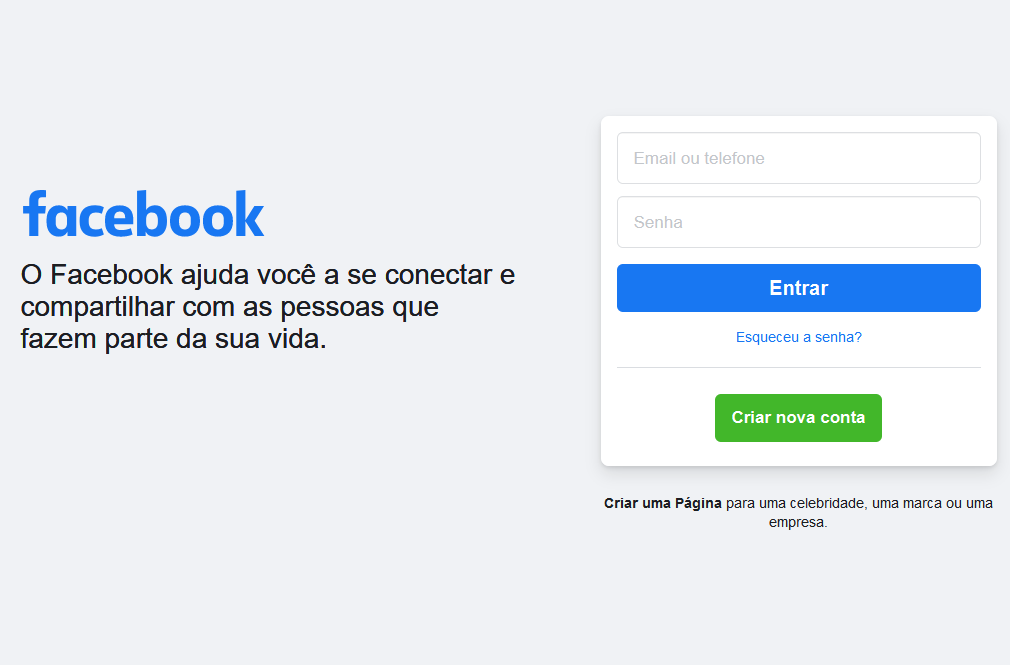
\includegraphics[width=\textwidth]{img/facebook.png}
    \caption{A página de login do facebook, exigindo seu email e senha.}
    \label{fig:facebook}
\end{figure}

Os mecanismos de segurança se baseiam em reconhecer a pessoa que quer acessar a informação. Ela se reduz basicamente a dois conceitos que tornam isso possível:

\begin{itemize}
    \item Algo que só você sabe
    \item Algo que só você tem
\end{itemize}

\subsection{Algo que só você sabe}

Esses são basicamente as senhas e perguntas que você faz a uma pessoa para identificá-la. Se alguém que quer se autenticar oferece corretamente a senha ou as respostas das perguntas que você faz a ela, você sabe que é quem diz ser.

Perguntas e respostas são um método bem rudimentar, já que alguém pode escavar a informação e descobrir resposta. Senhas também não são a melhor coisa do mundo. Senhas grandes são difíceis de memorizar e senhas pequenas são fáceis de serem descobertas. É tentador usar a mesma senha para tudo, só que se você fizer isso estará colocando todos os ovos na mesma cesta, e criando uma vulnerabilidade. 

% TODO: colocar referência ao cap 3
Falaremos mais de senhas no capítulo 3.

\subsection{Algo que só você tem}

Isto é, algo único que você tem. O que vem mais a mente é as digitais. Sua digital é praticamente única e um leitor de digital é extremamente prático em diversas situações. Pode ser usado outros tipos de identificação biométrica como a de iris e a de rosto inteiro.

Outro tipo de identificação dessa forma é a do seu celular, muito usado em autorização em duas etapas. Seu celular tem um número de série único, IMEI único e outros tipos de identificação de hardware que podem ser utilizados para sua verificação.

\begin{saibamais}
\subsection*{Hardware}

A parte eletrônica e física real do computador ou celular. São as peças que compõe a máquina, telas, caixas de som, processadores, drives, baterias, etc... \\

\subsection*{Software}

Os Software são os programas de computador. Eles não existem fisicamente e comandam o computador. É composto de todas as sequências e instruções digitais que dirigem a forma com você interage com a máquina. É armazenado digitalmente, muitas vezes no próprio computador que o utiliza.

A palavra vem do inglês, sendo um trocadilho com Hardware, onde o hard (Que significa rígido, forte) é trocado por soft (Macio). Como ware significa ferramenta, software traduz para: "Ferramenta Macia".

\end{saibamais}

\subsection{Ambos}

Uma combinação de ambos os métodos acima é ideal para sua proteção. Muitos sites oferecem, e até exigem, que você use os dois, o chamado de \textbf{Verificação em duas etapas}. Vai ser muito difícil alguém conseguir as duas formas de verificação ao mesmo tempo se você usá-la. Se alguém descobrir sua senha ainda vai precisar de seu celular para conseguir entrar na sua conta, e se ela roubar seu celular ainda vai precisar descobrir a sua senha, portanto é uma forma bem resiliente de proteção.

\section{Conclusão}

Neste capítulo vimos a importância da privacidade e da necessidade de protegê-la. Também vimos como categorizar e identificar vulnerabilidades e ameaças de segurança. No final identificamos o que torna algo seguro através de reconhecer as formas de identificação confiável através de algo que você sabe e algo que você tem.

\chapter{Exercícios}

\subsection*{Exercício 1}

Responda as perguntas abaixo:

\begin{enumerate}
    \item Porquê a noção da privacidade é necessária?
    \item Qual é a lei que oferece no brasil os direitos de proteção de dados? O que ela tem como fundamentos?
    \item Quais são os tipos de vulnerabilidade? Cite exemplos de vulnerabilidades digitais fáceis de se tomar preucauções.
\end{enumerate}

\subsection*{Exercício 2}

Marque verdadeiro ou falso nas questões abaixo:

\begin{enumerate}
    \item ( ) Incêndio causado por falha elétrica é considerado uma causa natural.
    \item ( ) Vírus de computador são ameaças do tipo lógicas.
\end{enumerate}
